\chapter{Kiến Trúc \& Topology Hệ Thống}
\label{ch:architecture}

\section{Tổng quan kiến trúc đám mây AWS}
Hệ thống được thiết kế và triển khai trên nền tảng đám mây công cộng Amazon Web Services (AWS) tại Region Singapore (\texttt{ap-southeast-1}). Kiến trúc tuân thủ nguyên tắc phòng thủ đa lớp (\textit{Defense-in-Depth}) kết hợp mô hình không tin cậy (\textit{Zero-Trust Architecture}), phân tách rõ ràng giữa phân vùng mạng biên tiếp nhận lưu lượng truy cập công cộng và vùng mạng nội bộ bảo vệ các máy chủ chứa dữ liệu và ứng dụng vi dịch vụ.

\begin{figure}[H]
    \centering
    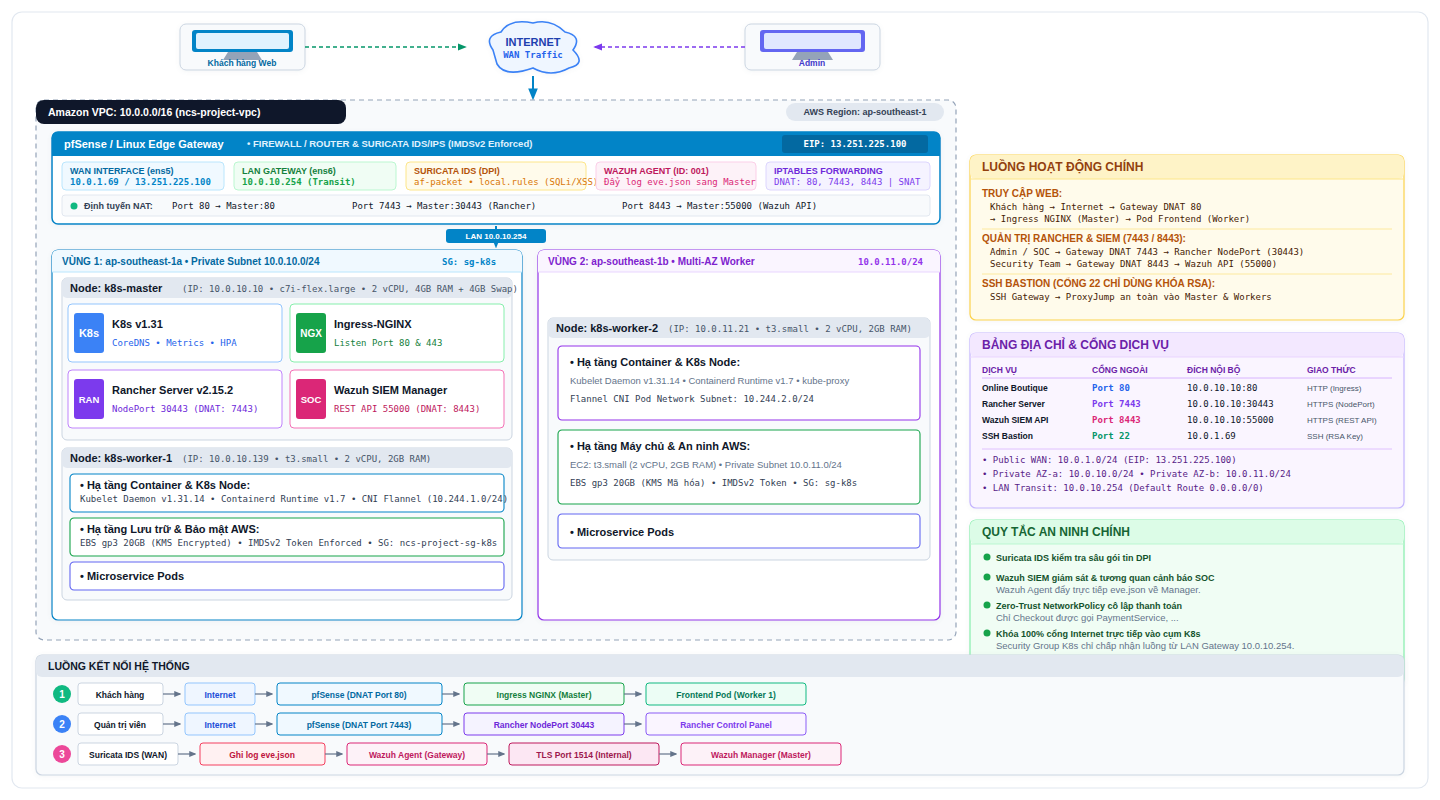
\includegraphics[width=\textwidth]{images/architecture_diagram.png}
    \caption{Sơ đồ kiến trúc tổng thể hệ thống an ninh hạ tầng Microservices trên AWS}
    \label{fig:architecture_diagram}
\end{figure}

\section{Bảng tóm tắt các dịch vụ ứng dụng triển khai}
Ứng dụng thương mại điện tử Google Online Boutique bao gồm 11 vi dịch vụ độc lập kết hợp cùng 1 dịch vụ sinh tải (\texttt{loadgenerator}). Các dịch vụ được đóng gói dưới dạng container Docker, vận hành trên cụm Kubernetes v1.31 và giao tiếp nội bộ qua giao thức gRPC hiệu năng cao hoặc HTTP REST:

\begin{table}[H]
    \centering
    \small
    \renewcommand{\arraystretch}{1.2}
    \caption{Bảng tóm tắt các dịch vụ ứng dụng Online Boutique triển khai trên cụm K8s}
    \label{tab:services_summary}
    \begin{tabularx}{\textwidth}{l l c l X}
        \toprule
        \textbf{Dịch vụ (Service)} & \textbf{Ngôn ngữ} & \textbf{Cổng} & \textbf{Giao thức} & \textbf{Vai trò chức năng} \\
        \midrule
        \texttt{frontend} & Go & 80 & HTTP & Giao diện web người dùng, hiển thị trang chủ và sản phẩm \\
        \texttt{cartservice} & C\# (.NET) & 7070 & gRPC & Quản lý thông tin giỏ hàng của từng phiên người dùng \\
        \texttt{redis-cart} & Redis & 6379 & TCP & Bộ nhớ đệm in-memory lưu trữ tạm thời giỏ hàng \\
        \texttt{productcatalogservice} & Go & 3550 & gRPC & Cung cấp danh mục sản phẩm, tìm kiếm và chi tiết món đồ \\
        \texttt{checkoutservice} & Go & 5050 & gRPC & Tiếp nhận đơn hàng, điều phối thanh toán và gửi email \\
        \texttt{paymentservice} & Node.js & 50051 & gRPC & Xử lý thanh toán thẻ tín dụng (bảo vệ bởi Zero-Trust NetPol) \\
        \texttt{currencyservice} & Node.js & 7000 & gRPC & Chuyển đổi và tính toán tỷ giá ngoại tệ theo thời gian thực \\
        \texttt{emailservice} & Python & 8080 & gRPC & Soạn thảo và gửi email xác nhận đặt hàng thành công \\
        \texttt{shippingservice} & Go & 50051 & gRPC & Tính cước phí vận chuyển và xuất mã vận đơn giao hàng \\
        \texttt{recommendationservice} & Python & 8080 & gRPC & Đề xuất gợi ý các sản phẩm liên quan theo ngữ cảnh \\
        \texttt{adservice} & Java & 9555 & gRPC & Hiển thị các mẩu tin quảng cáo và khuyến mãi sản phẩm \\
        \texttt{loadgenerator} & Python & -- & HTTP & Giả lập lưu lượng truy cập liên tục để kích hoạt HPA \\
        \bottomrule
    \end{tabularx}
\end{table}

\section{Phân vùng mạng và định tuyến (VPC \& Subnets)}
Toàn bộ hạ tầng mạng được bao bọc trong một đám mây ảo riêng biệt \textbf{Amazon VPC} (\texttt{ncs-project-vpc}) với dải mạng \texttt{10.0.0.0/16}. Hạ tầng mạng được chia thành 3 Subnet chính trải dài trên 2 Vùng sẵn sàng (\textit{Availability Zones - AZ}) nhằm đảm bảo khả năng chịu lỗi và tính sẵn sàng cao:

\begin{table}[H]
    \centering
    \small
    \renewcommand{\arraystretch}{1.25}
    \caption{Bảng phân bổ không gian địa chỉ IP và Subnet trên AWS}
    \label{tab:subnets}
    \begin{tabularx}{\textwidth}{l l l l X}
        \toprule
        \textbf{Tên Subnet} & \textbf{Vùng AZ} & \textbf{Dải CIDR} & \textbf{Loại mạng} & \textbf{Mục đích sử dụng} \\
        \midrule
        \texttt{public-subnet} & \texttt{ap-southeast-1a} & \texttt{10.0.1.0/24} & Public & Chứa Edge Gateway, tiếp nhận lưu lượng từ Internet \\
        \texttt{private-subnet-a} & \texttt{ap-southeast-1a} & \texttt{10.0.10.0/24} & Private & Cụm K8s Master và Worker 1 \\
        \texttt{private-subnet-b} & \texttt{ap-southeast-1b} & \texttt{10.0.11.0/24} & Private & Cụm K8s Worker 2 (Phân tán tải Multi-AZ Worker) \\
        \bottomrule
    \end{tabularx}
\end{table}

\subsection{Cơ chế định tuyến bảng định tuyến (Route Tables)}
\begin{enumerate}
    \item \textbf{Public Route Table}: Gắn trực tiếp với \textit{Internet Gateway} (\texttt{igw}). Định tuyến \texttt{0.0.0.0/0} hướng thẳng ra \texttt{igw}, cho phép Gateway tiếp nhận lưu lượng Internet thông qua địa chỉ IP tĩnh co giãn duy nhất \textbf{Elastic IP (EIP: \texttt{13.251.225.100})}.
    \item \textbf{Private Route Table}: Được liên kết với cả 2 Subnet nội bộ (\texttt{10.0.10.0/24} và \texttt{10.0.11.0/24}). Quy tắc \texttt{0.0.0.0/0} được cấu hình trỏ đích đến Network Interface LAN (\texttt{ens6} - IP: \texttt{10.0.10.254}) của máy chủ Gateway. Cơ chế này ép buộc toàn bộ lưu lượng Egress từ cụm Kubernetes đi ra Internet để cập nhật gói phần mềm hay kéo Image container đều phải đi qua Gateway để được kiểm duyệt.
\end{enumerate}

\section{Nhóm an ninh (Security Groups) và Kiểm soát truy cập}
Hạ tầng áp dụng 2 Security Group độc lập nhằm thực hiện nguyên tắc đặc quyền tối thiểu (\textit{Least Privilege}):
\begin{itemize}
    \item \textbf{\texttt{ncs-project-sg-pfsense}}: Áp dụng cho máy chủ Edge Gateway. Mở các cổng công khai từ Internet: cổng 80 (HTTP), cổng 443 (HTTPS), cổng 7443 (Rancher Manager), cổng 8443 (Wazuh SIEM API) và cổng 22 (SSH Bastion hạn chế).
    \item \textbf{\texttt{ncs-project-sg-k8s}}: Áp dụng cho Master node và Worker nodes. \textbf{Khóa hoàn toàn mọi truy cập trực tiếp từ Internet}. Chỉ chấp nhận lưu lượng chuyển tiếp nội bộ đến từ card mạng LAN của Gateway (\texttt{10.0.10.254}) và cho phép thông suốt toàn bộ lưu lượng nội bộ giữa các Node trong dải \texttt{10.0.0.0/16}.
\end{itemize}

\section{Bảng ánh xạ cổng dịch vụ và cơ chế NAT (Port Mapping Table)}
Để người dùng và quản trị viên có thể truy cập tất cả các dịch vụ độc lập thông qua \textbf{duy nhất một địa chỉ IP Public (\texttt{13.251.225.100})} mà không xảy ra xung đột, Gateway sử dụng kỹ thuật \textit{Destination NAT (DNAT)} kết hợp \textit{Source NAT (Masquerade)}:

\begin{table}[H]
    \centering
    \small
    \renewcommand{\arraystretch}{1.25}
    \caption{Bảng phân bổ cổng dịch vụ và quy tắc chuyển tiếp NAT}
    \label{tab:port_mapping}
    \begin{tabularx}{\textwidth}{l c c l X}
        \toprule
        \textbf{Tên Dịch Vụ} & \textbf{Cổng Ext} & \textbf{Giao thức} & \textbf{Đích Internal (DNAT)} & \textbf{Mô Tả Chức Năng} \\
        \midrule
        \textbf{Online Boutique} & \textbf{80} & HTTP & \texttt{10.0.10.10:80} & Ứng dụng web thương mại điện tử \\
        \textbf{Rancher Server} & \textbf{7443} & HTTPS & \texttt{10.0.10.10:30443} & Giao diện quản trị tập trung cụm K8s \\
        \textbf{Wazuh SIEM} & \textbf{8443} & HTTPS & \texttt{10.0.10.10:55000} & Giao tiếp REST API \& Giám sát an ninh \\
        \textbf{SSH Bastion} & \textbf{22} & SSH & Trực tiếp tại Gateway & Quản trị dòng lệnh máy chủ qua khóa RSA \\
        \bottomrule
    \end{tabularx}
\end{table}

\section{Mạng Pod Overlay (Flannel VXLAN)}
Cụm Kubernetes sử dụng giải pháp CNI \textbf{Flannel} hoạt động trên chế độ \texttt{vxlan} với không gian địa chỉ Pod CIDR là \texttt{10.244.0.0/16}:
\begin{itemize}
    \item Mỗi node trong cụm được phân bổ một không gian con \texttt{/24} (ví dụ: Master \texttt{10.244.0.0/24}, Worker 1 \texttt{10.244.1.0/24}, Worker 2 \texttt{10.244.2.0/24}).
    \item Gói tin trao đổi giữa các Pod được đóng gói trong giao thức UDP port 8472 trên card mạng nội bộ, cho phép các Pod thuộc 12 vi dịch vụ giao tiếp liền mạch xuyên suốt giữa 2 Vùng sẵn sàng (\texttt{ap-southeast-1a} và \texttt{ap-southeast-1b}) mà không bị giới hạn bởi cấu trúc định tuyến vật lý của AWS VPC.
\end{itemize}

\section{Phân bổ tài nguyên máy chủ EC2}
Hệ thống được thiết kế và phân bổ cấu hình máy chủ ảo Amazon EC2 tối ưu, đảm bảo đáp ứng đầy đủ năng lực tính toán và bộ nhớ cho cả cụm Kubernetes lẫn các thành phần giám sát an ninh:

\begin{table}[H]
    \centering
    \small
    \renewcommand{\arraystretch}{1.25}
    \caption{Bảng phân bổ tài nguyên máy chủ EC2 trong hệ thống}
    \label{tab:ec2_resources}
    \begin{tabularx}{\textwidth}{l l c c c X}
        \toprule
        \textbf{Máy chủ (Host)} & \textbf{Loại Instance} & \textbf{vCPU} & \textbf{RAM} & \textbf{EBS Disk} & \textbf{Nhiệm vụ chính} \\
        \midrule
        \texttt{pfsense-gateway} & \texttt{t3.small} & 2 & 2 GB & 20 GB (gp3) & Gateway, Suricata IDS, NAT, Bastion \\
        \texttt{k8s-master} & \texttt{c7i-flex.large} & 2 & 4 GB & 20 GB (gp3) & K8s Control Plane, Ingress, Rancher, Wazuh \\
        \texttt{k8s-worker-1} & \texttt{t3.small} & 2 & 2 GB & 20 GB (gp3) & K8s Worker node (Kube-Scheduler tự động điều phối Pods) \\
        \texttt{k8s-worker-2} & \texttt{t3.small} & 2 & 2 GB & 20 GB (gp3) & K8s Worker node Multi-AZ (Cân bằng tải song song, chịu lỗi) \\
        \midrule
        \multicolumn{2}{l}{\textbf{Tổng cộng tài nguyên}} & \textbf{8} & \textbf{10 GB} & \textbf{80 GB} & \textbf{4 Máy chủ vận hành ổn định} \\
        \bottomrule
    \end{tabularx}
\end{table}
